\section{Sensor \& Hardware Board}
\begin{frame}
	\frametitle{Vorgaben an Sensor und Hardware-Board}
	\begin{itemize}
		\item Keine mechanischen Veränderungen an der zu messenden Uhr zulässig.
		\item Verschiedene Pendeltypen müssen erkennbar sein.
		\item Hard- Realtime System mit höchsten Anforderungen an Zeitkonstanz.
		\item Verzögerungen müssen immer gleich gross sein.
	\end{itemize}
\end{frame}

\subsection{Sensor}
\begin{frame}
	\frametitle{Eigenschaften des Sensors}
	\begin{minipage}{0.65\textwidth}
		\begin{itemize}
			\item Reflektions-Lichtschranke mit Infrarot-Lichtstrahl.
			\item Sender und Empfänger vereinigt mit kleinem Abstand.
			\item SMD Element mit 6.2 x 4.2mm Platzbedarf.
			\item Maximal $50\mu s$ Abfallzeit der Spannung.
			\item Analoger Sensor verlangt erweiterte Schaltung.
		\end{itemize}
	\end{minipage}
	\begin{minipage}[r]{0.25\textwidth}
		\centering
		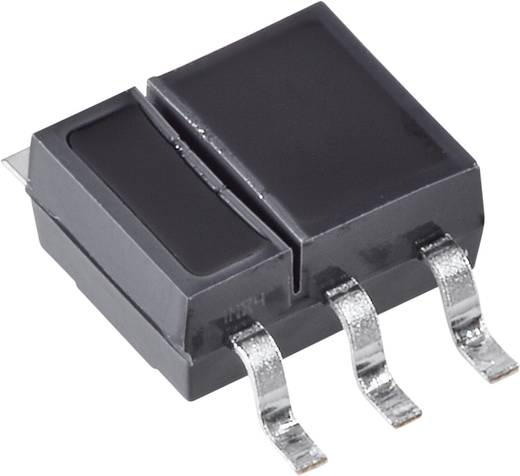
\includegraphics[width=\textwidth]{../docs/images/reflexions-lichtschranke-sfh91019201-osram-1-st}
	\end{minipage}
\end{frame}

\begin{frame}
	\frametitle{Schema des Sensor Boards}
	\begin{itemize}
		\item Einstellbare Schaltgrenzen für unterschiedlich reflektierende Pendel.
		\item Schmitt- Trigger für eindeutige Zustände High / Low.
		\item LED zur visuellen Überprüfung der Schaltung.
	\end{itemize}
	\centering
	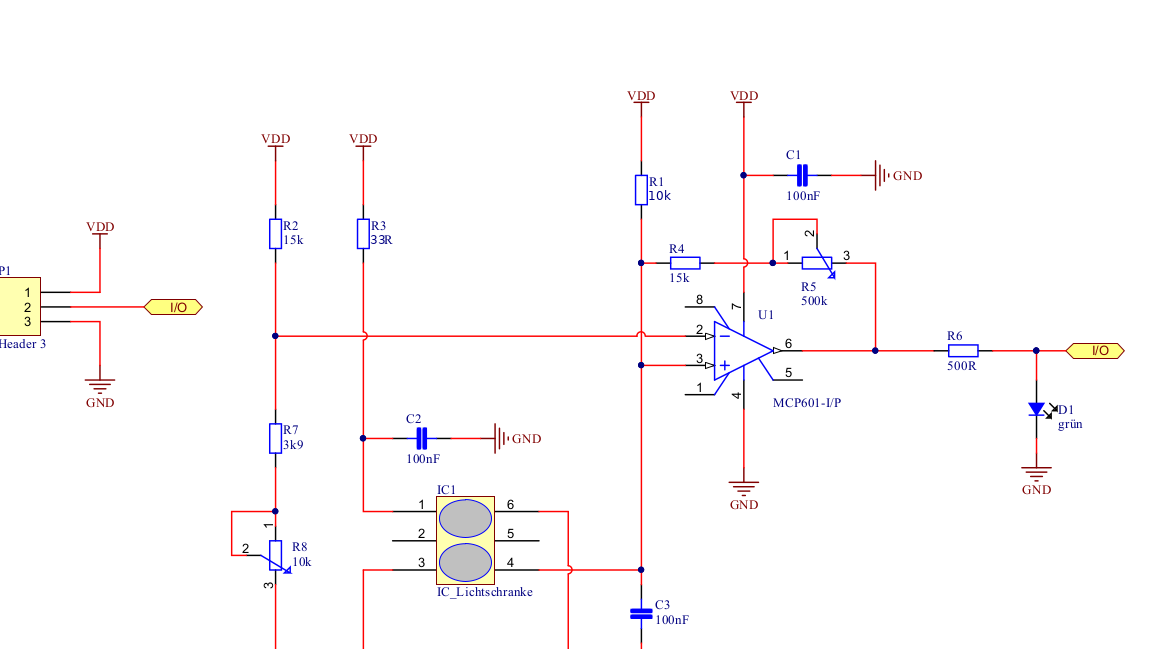
\includegraphics[width=0.7\textwidth]{../docs/images/Circuit_Sensor}
\end{frame}

\begin{frame}
	\frametitle{Aufbau der Messeinheit mit Sensor}
	\begin{minipage}{0.45\textwidth}
		\begin{itemize}
			\item Schlanke Bauweise um wenig Platz zu beanspruchen.
			\item Gewichte erschweren ein Kippen der Einheit.
			\item Höhe im 10mm Raster, Abstand stufenlos verstellbar.
		\end{itemize}
		\centering
		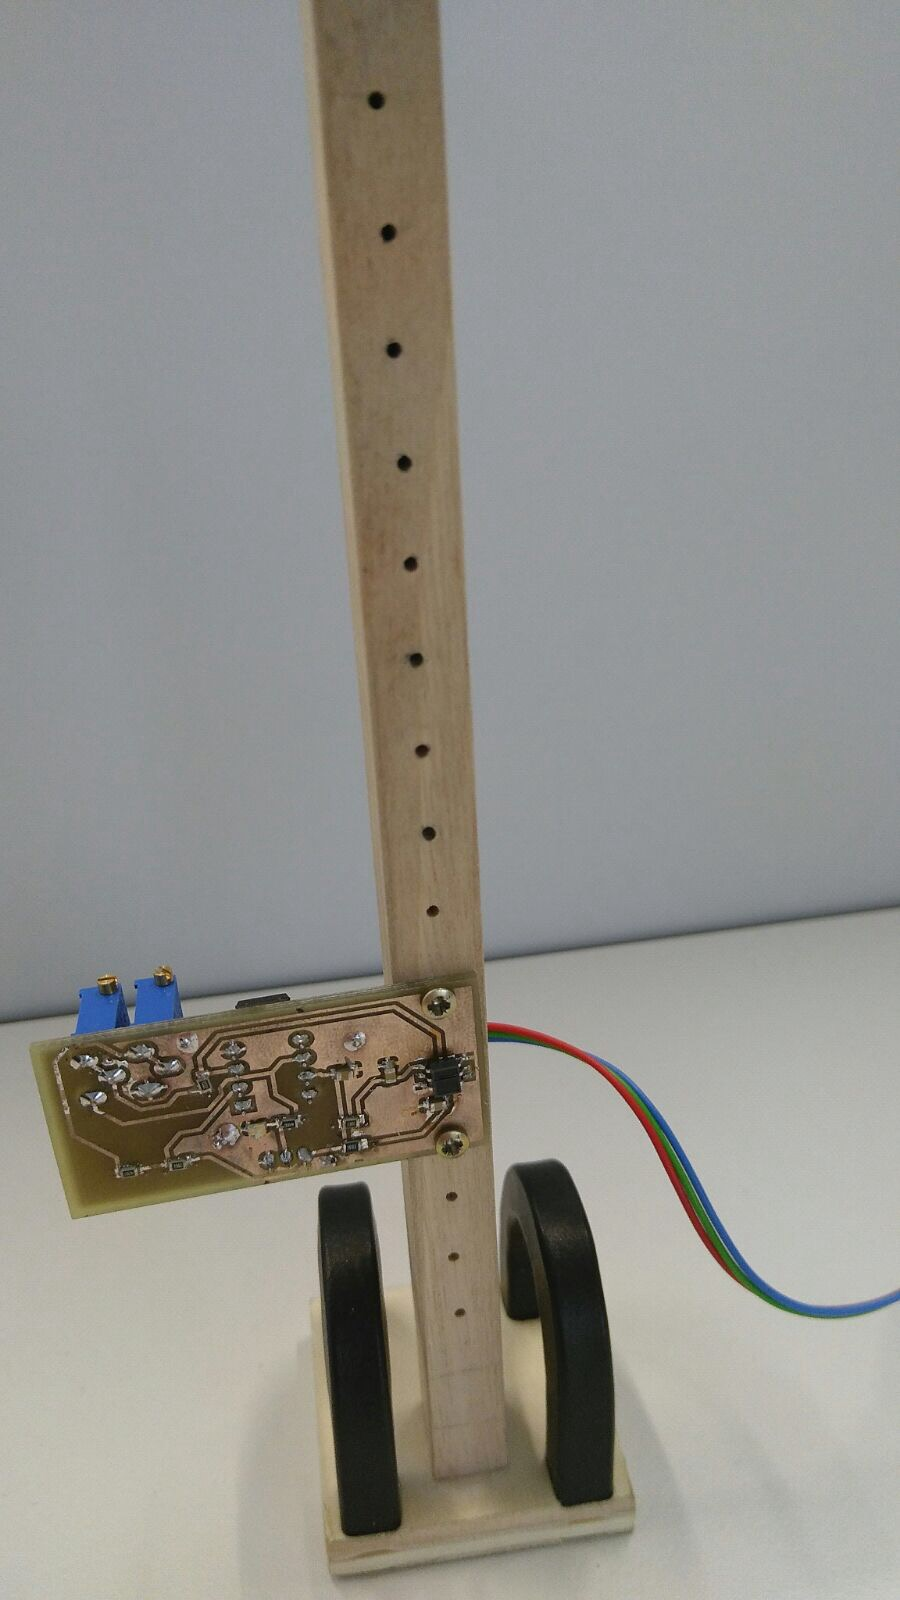
\includegraphics[width=0.25\textwidth]{../docs/images/Sensor_FullView}
	\end{minipage}
	\begin{minipage}{0.45\textwidth}
		\begin{itemize}
			\item Potentiometer auch während der Messung zugänglich.
			\item Sensor befindet sich mittig vor dem Ständer.
			\item Elemente vor Spannungsschwankungen geschützt.
		\end{itemize}
		\centering
		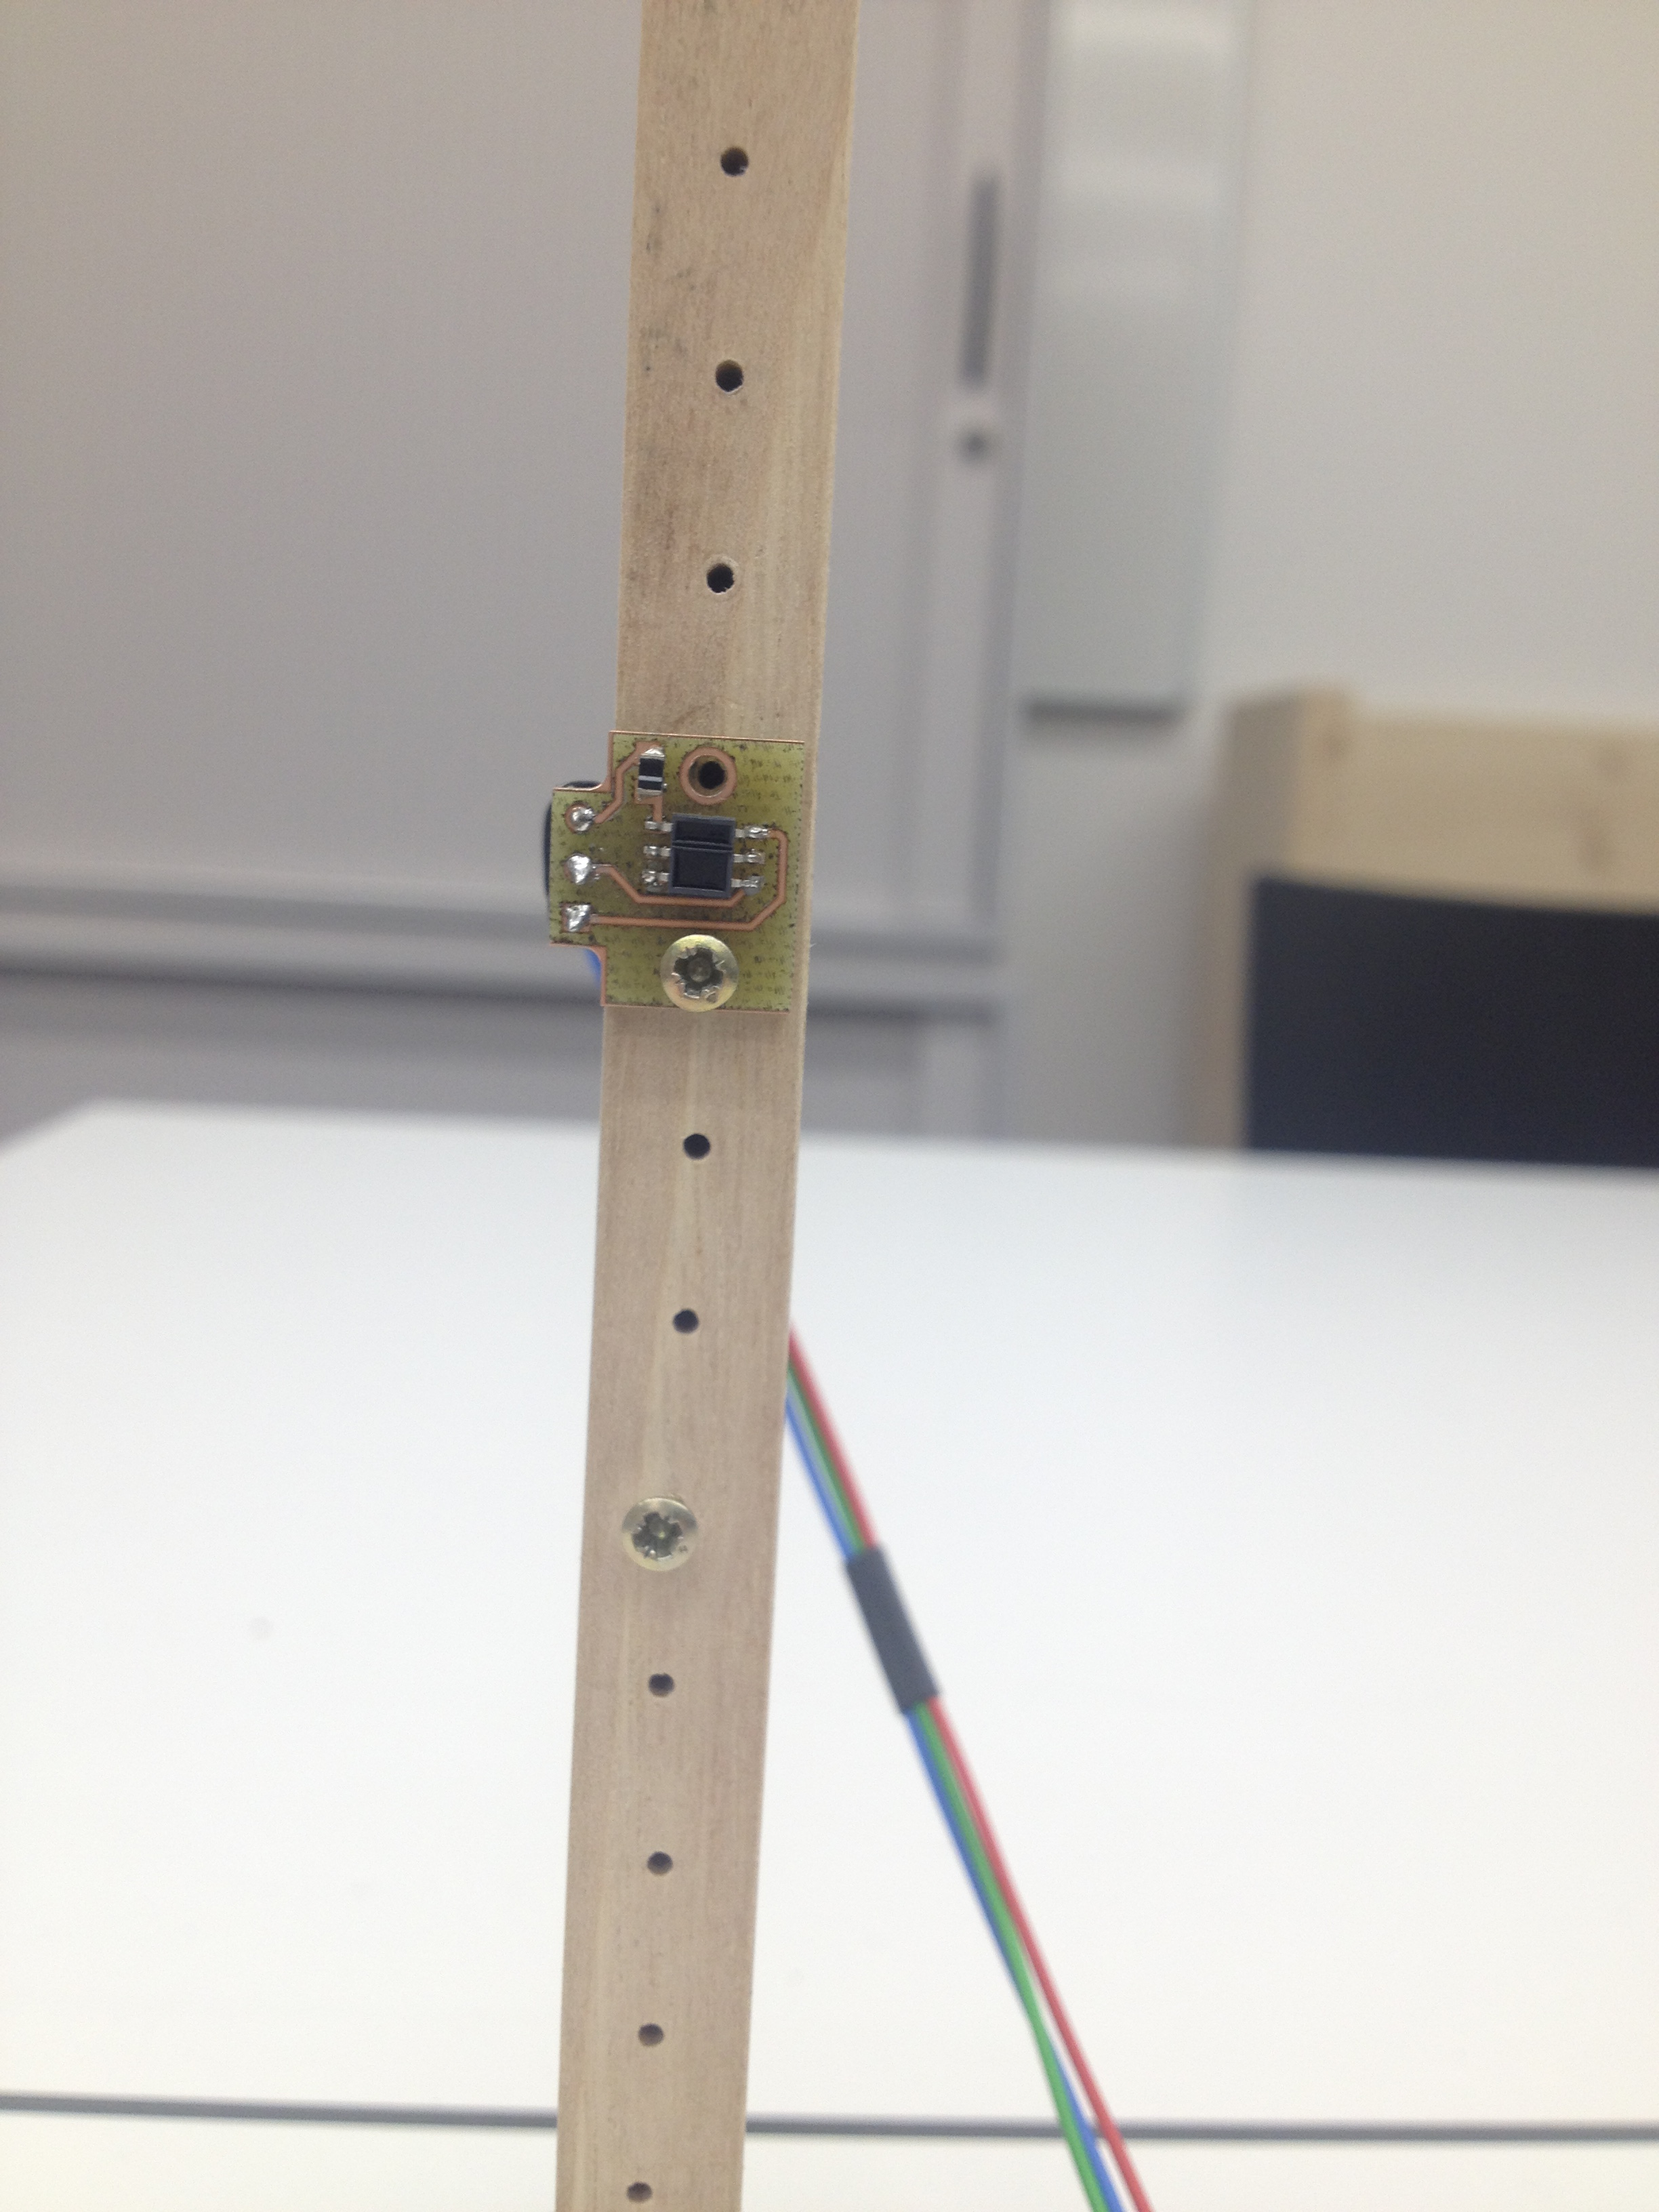
\includegraphics[width=0.75\textwidth]{../docs/images/Sensor_Detail}
	\end{minipage}
\end{frame}

\subsection{Hardware Board}
\begin{frame}
	\frametitle{Übersicht Hardware Board}
	\begin{minipage}{0.45\textwidth}
		\begin{itemize}
			\item GPS-Modul zur Disziplinierung des Systems mittels Sekundenpuls.
			\item Real Time Clock für die Systemzeit (optional).
			\item Tiny K20 Mikrocontroller- Board für die Auswertung der Daten.
			\item Kommunikation zum Raspberry Pi mittels USB und UART-RS232.
			\item Software in C mit Hilfe von Processor Expert.
		\end{itemize}
	\end{minipage}
	\begin{minipage}{0.45\textwidth}
		\centering
		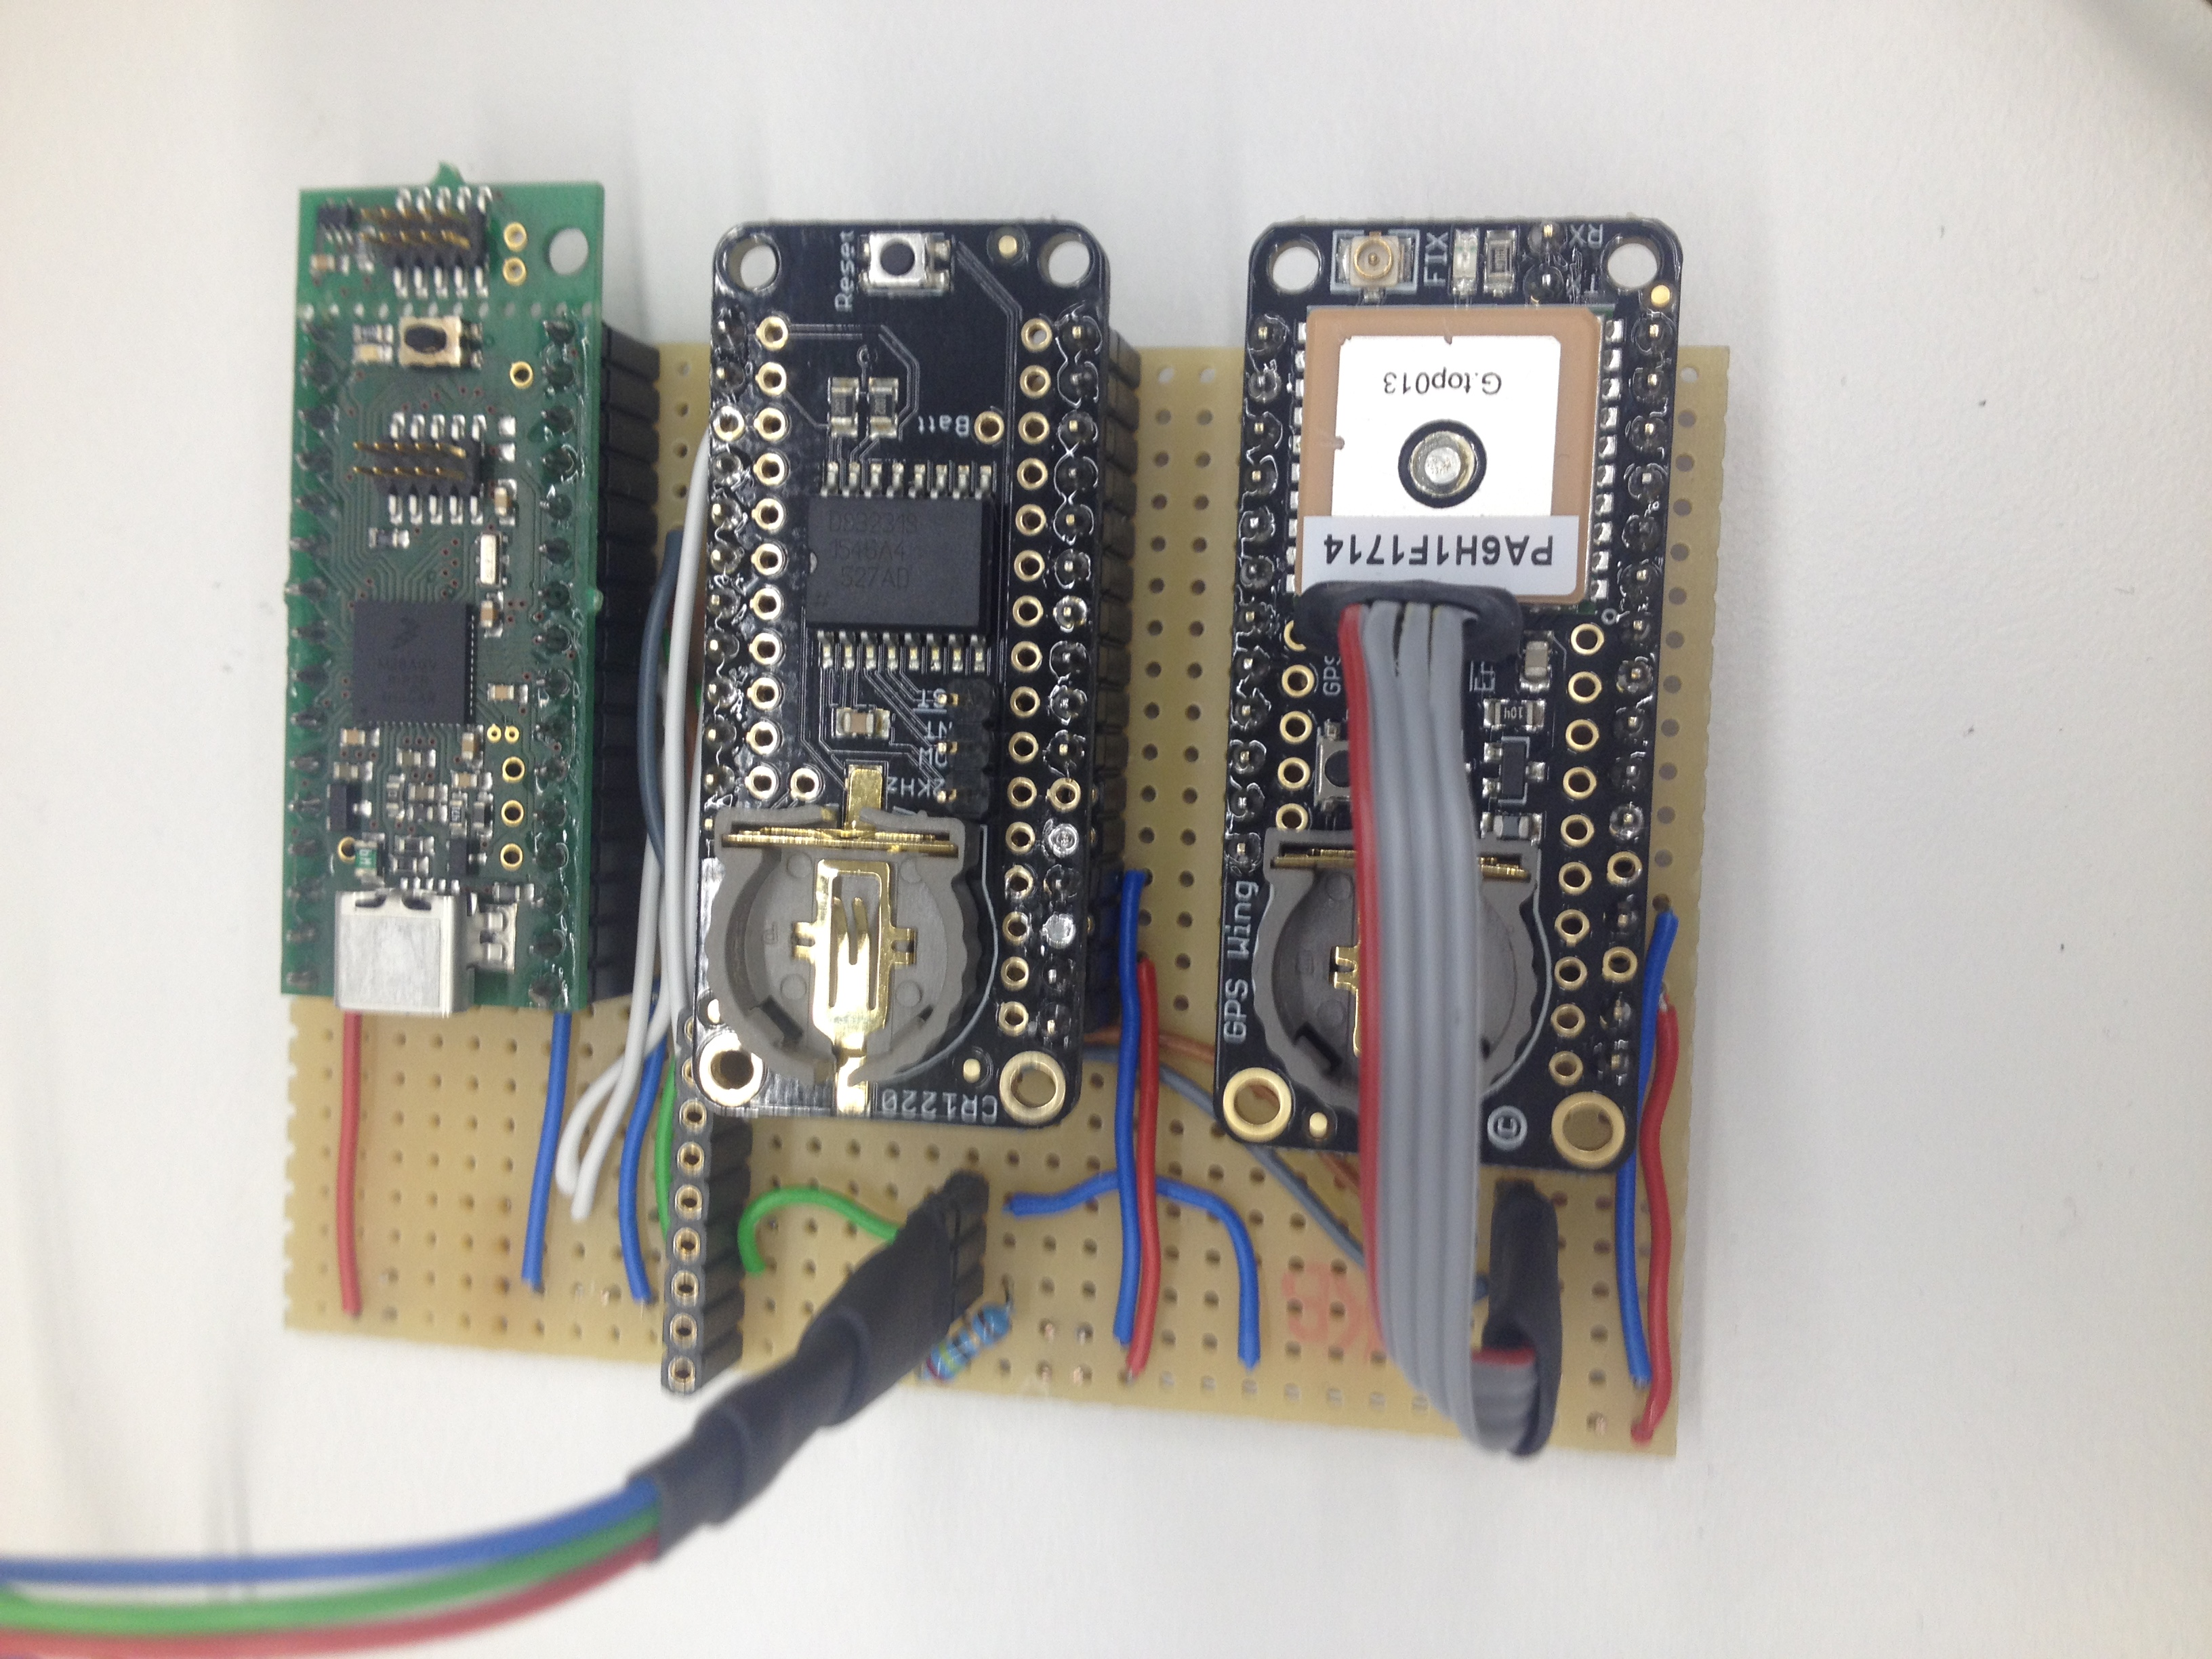
\includegraphics[width=\textwidth]{../docs/images/HW_Board_Complete}
	\end{minipage}
\end{frame}

\subsection{Ablauf der Messung}
\begin{frame}
	\frametitle{Beschrieb des Zusammenspiels}
	\begin{itemize}
		\item Hardwarezähler getrieben vom Kristall des Tiny K20.
		\item GPS-Modul liefert ein Puls pro Sekunde (PPS) und löst Interrupt aus.
		\item Referenzfrequenz = Zählerwert bei PPS - letzter Zählerwert bei PPS.
		\item Sensor löst bei Schaltung ebenfalls ein Interrupt aus.
		\item Pendelzeit = Zählerwert bei Sensor-Interrupt - letzter Sensorzählerwert.
		\item Auswerten und versenden der Daten zwischen den Interrupts.
	\end{itemize}
\end{frame}

\begin{frame}
	\frametitle{Sequenzdiagramm des Zusammenspiels}
	\centering
	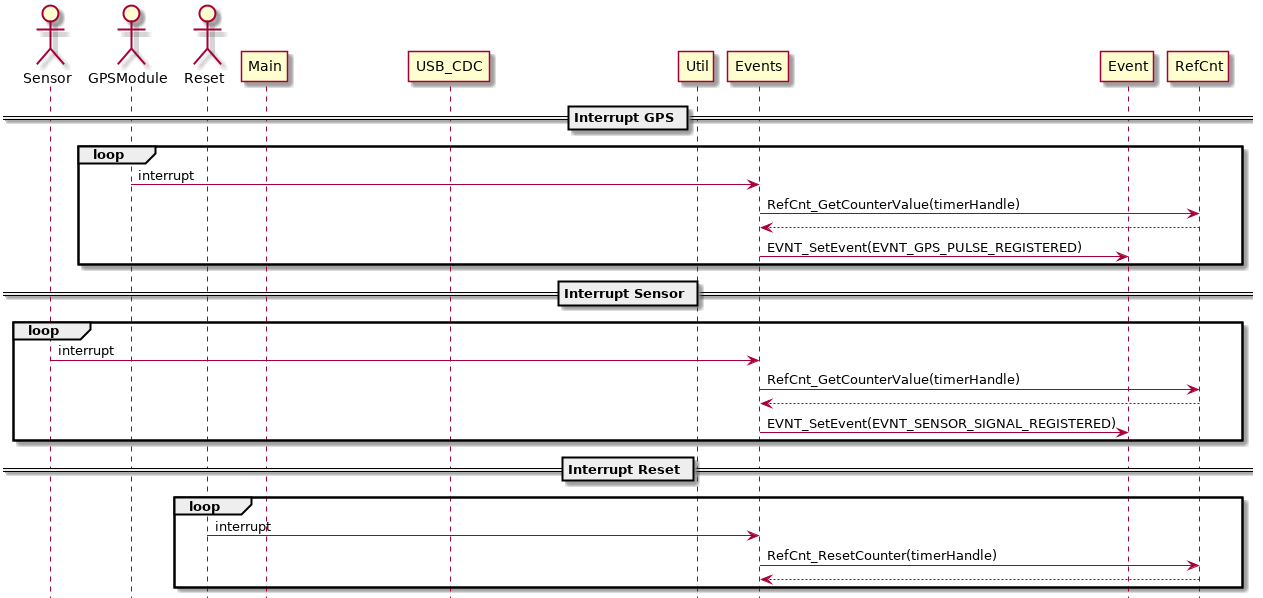
\includegraphics[width=\textwidth]{../docs/uml/sequence_hwb_1}
\end{frame}

\begin{frame}
	\frametitle{Sequenzdiagramm des Zusammenspiels}
	\centering
	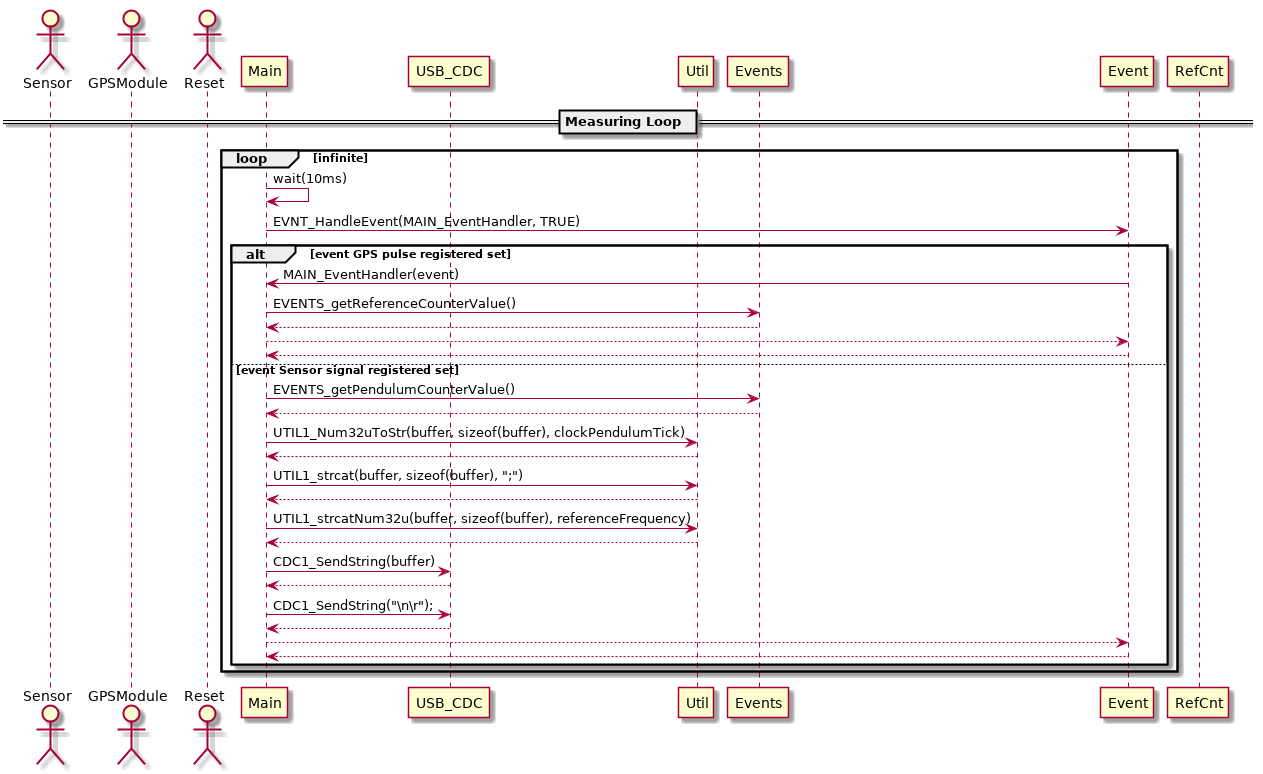
\includegraphics[width=\textwidth]{../docs/uml/sequence_hwb_2}
\end{frame}